\documentclass{beamer}
\def\java{\texttt{Java}}
\def\mytoday{2 November 2016}
\usepackage{pgfpages}\def\mpause{\pause}
%\usepackage{pgfpages}\pgfpagesuselayout{8 on 1}[a4paper,border shrink=1mm, landscape]\def\mpause{}
\usepackage{url}
\usepackage{verbatim}
\usepackage{color}
\usepackage{listings}
\usepackage{code}
\usepackage{textcomp}
%\usepackage{epsfig}
\usepackage{graphicx}
\def\bu{\vspace{1ex}\par$\bullet$\hspace{2ex}}

%\usepackage{bm}
\usepackage{beamerthemesplit}
\defbeamertemplate*{footline}{infolines theme}{
\hspace*{2ex}    \insertframenumber{} / \inserttotalframenumber\hspace*{2ex} 
\copyright Manfred Kerber
%   \insertpagenumber{} / \insertpresentationendpage \hspace*{2ex}
  \vskip1ex}

\def\mcolor#1#2{\rule{0ex}{0ex}\color{#1}#2\color{black}{}}
\usetheme{Copenhagen}
%\setbeamercolor{title}{fg=red!80!black,bg=red!20!white}
\makeatletter % code block to allow custom labels to be cross-ref'ed; see comp.text.tex "customized display labels cross-ref'd"
\begin{document}

\title{MSc/ICY Software Workshop\\
Classes and Inheritance}

\author[Manfred~Kerber]{\begin{tabular}{ll}
\mcolor{blue}{Manfred Kerber} &   {\tt www.cs.bham.ac.uk/\~{}mmk}\\
\end{tabular}}

\date{\mytoday}

\begin{frame}
\titlepage
\end{frame}

\begin{frame}
\frametitle{Object-Oriented Programming}
Distinguish:

\begin{itemize}
\item \mcolor{blue}{\bf Classes}, e.g., \texttt{BankAccount}, \texttt{Customer}
\item \mcolor{blue}{\bf Objects}, e.g., \texttt{bankAccountJohn}, \texttt{customerMary}\\
 created by a \mcolor{blue}{\bf Constructor}, e.g.\\
    \texttt{public BankAccount (Customer customer, String password)}
\item \mcolor{blue}{\bf Methods}, e.g.  \texttt{getBalance()}
\end{itemize}
\end{frame}


\begin{frame}
\frametitle{Superclass vs subclass}

\begin{itemize}
\item A subclass \mcolor{blue}{\texttt{SubclassA}} inherits from its (unique)
  superclass \mcolor{blue}{\texttt{SuperclassB}} (introduced by
  \mcolor{blue}{\texttt{public class SubclassA extends SuperclassB}})

\item All methods not explicitly overridden in the subclass are inherited from the superclass.

\item Overridden methods from the superclass are accessible via
  \texttt{super} in the body of the overriding method, e.g., in
  writing the code for a \texttt{toString()} method you can use
  \mcolor{blue}{\texttt{super.toString()}}.

\item Variables (and methods) private to the superclass are
  \mcolor{blue}{not accessible} from the subclass.
\end{itemize}
\end{frame}

\begin{frame}
\frametitle{Rationale for Inheritance}

\mcolor{blue}{Inheritance is a very important feature of object
  oriented programming.}

\begin{itemize}
  \item Inherit methods, that is, methods that are common to the
    superclass can be used without duplication of code.
  \item Inheritance keeps code simpler.
  \item If code needs to be changed (and remember very often it needs
    to be changed) then it can be changed at a \mcolor{blue}{single
      point}. This is important since it makes code maintainable (if
    code is duplicated any changes may be messy since parts may be
    overlooked and inconsistencies may be introduced).
\end{itemize}

\end{frame}

\begin{frame}
\frametitle{Example: rudimentary library system}

\begin{itemize}
\item The library offers books on loan, either on
  \mcolor{blue}{\texttt{shortLoan}} (one day) or
  \mcolor{blue}{\texttt{longLoan}} (at most 30 days)
\item \mcolor{blue}{\texttt{User}}s are either
  \mcolor{blue}{\texttt{StudentUser}},
  \mcolor{blue}{\texttt{StaffUser}}, or
  \mcolor{blue}{\texttt{CommunityUser}}.
\item Assume that students can borrow at most 10 books, staff and
  members of the community as many as they like. Members of the
  community have to pay a fee of \pounds~1 per book (others
  not). \mcolor{blue}{\texttt{UGUser}}s can borrow books for at
  most 10 days, \mcolor{blue}{\texttt{MScUser}}s for at most 20
  days, \mcolor{blue}{\texttt{PhDUser}}s for at most 30 days.
\end{itemize}
\end{frame}

\begin{frame}
\frametitle{Hierarchy of super- and subclasses}
%\psfig{figure=super.eps,scale=0.45}
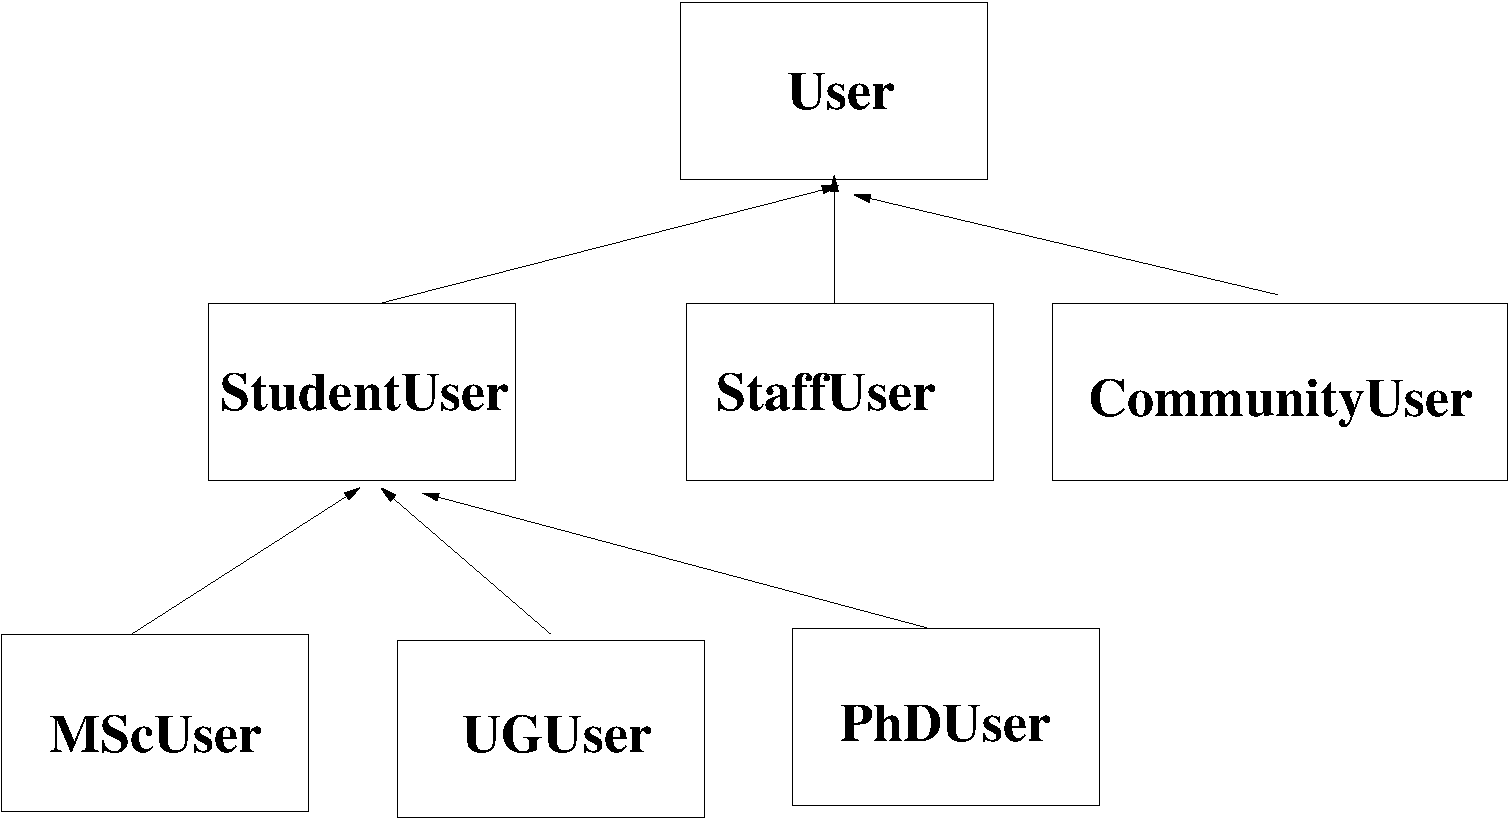
\includegraphics[height=.65\textheight]{super}
\end{frame}

\begin{frame}
\frametitle{Abstract Class}

E.g., \mcolor{blue}{\texttt{public abstract class User}}.

\mcolor{red}{Abstract classes do not have immediate objects, but only
  via subclasses.}

With an abstract class \mcolor{blue}{\texttt{User}}, with an abstract subclass
\mcolor{blue}{\texttt{StudentUser}} and (non-abstract) subclasses \mcolor{blue}{\texttt{StaffUser}},
and \mcolor{blue}{\texttt{CommunityUser}}\\ as well as the three subclasses of
\mcolor{blue}{\texttt{StudentUser}}:\\
\bu \mcolor{blue}{\texttt{UGUser}},
\bu \mcolor{blue}{\texttt{MScUser}}, and 
\bu \mcolor{blue}{\texttt{PhDUser}}\\
each user object generated should be member of a class
\mcolor{blue}{\texttt{UGStudent}}, \mcolor{blue}{\texttt{MScStudent}},
\mcolor{blue}{\texttt{PhDStudent}}, \mcolor{blue}{\texttt{StaffUser}},
or \mcolor{blue}{\texttt{CommunityUser}}.
\end{frame}


\begin{frame}
\frametitle{Classes}

\begin{itemize}\itemsep0pt
\item have an abstract class \mcolor{blue}{\texttt{User}}
\item distinguish three subclasses of users: \mcolor{blue}{\texttt{StudentUser}},
  \mcolor{blue}{\texttt{StaffUser}}, \mcolor{blue}{\texttt{CommunityUser}}, using inheritance.
\item distinguish three subclasses of \mcolor{blue}{\texttt{StudentUser}}: \mcolor{blue}{\texttt{UGUser}},
  \mcolor{blue}{\texttt{MScUser}}, \mcolor{blue}{\texttt{PhDUser}}, using inheritance.
\item For a \mcolor{blue}{\texttt{User}} we know their \mcolor{blue}{\texttt{firstName}},
  \mcolor{blue}{\texttt{surname}}, \mcolor{blue}{\texttt{phoneNumber}}, \mcolor{blue}{\texttt{booksOnLoan}}. Each
  \mcolor{blue}{\texttt{bookOnLoan}} goes with the \mcolor{blue}{\texttt{Book}}, the
  \mcolor{blue}{\texttt{DateTime}} when it was borrowed, and the \mcolor{blue}{\texttt{DateTime}}
  when it has to be given back.
\end{itemize}

Build suitable classes: \mcolor{blue}{\texttt{User}},  \mcolor{blue}{\texttt{StudentUser}},
  \mcolor{blue}{\texttt{StaffUser}}, \mcolor{blue}{\texttt{CommunityUser}} making use of inheritance to model the situation.

\end{frame}

\end{document}


%%% Local Variables: 
%%% mode: latex
%%% TeX-master: "slides"Superclasses
%%% End: 

